\documentclass[11pt]{article}

\usepackage[margin=1in]{geometry}
\usepackage[T1]{fontenc}
\usepackage[utf8]{inputenc}
\usepackage{lmodern}
\usepackage{amsmath,amssymb,amsfonts}
\usepackage{bm}
\usepackage{enumitem}
\usepackage{booktabs}
\usepackage{xcolor}
\usepackage{hyperref}
\usepackage{array}
\usepackage{longtable}
\usepackage{titlesec}
\usepackage{tikz}
\usetikzlibrary{positioning,shapes.misc,arrows.meta}

\hypersetup{
    colorlinks=true,
    linkcolor=blue,
    urlcolor=blue,
    citecolor=blue
}

\titleformat{\section}{\large\bfseries}{\thesection.}{0.5em}{}
\titleformat{\subsection}{\normalsize\bfseries}{\thesubsection.}{0.5em}{}

\title{\textbf{Meeting Notes: Exosuit-Assisted Learning, Contraction/Stability Ideas, and Lab Logistics}}
\author{}
\date{}

\begin{document}

\maketitle

\section*{Meeting Overview}
These notes summarize a discussion about:
\begin{itemize}[leftmargin=1.5em]
    \item modeling an exosuit/exoskeleton interaction with a human/manipulator,
    \item using stiffness/damping modulation as a feedback channel,
    \item contraction/stability-inspired control ideas,
    \item possible rehabilitation implications,
    \item simulation and implementation plans,
    \item paper direction and short-term milestones,
    \item and some separate lab/logistics discussion.
\end{itemize}

Because the source transcript was partially noisy, these notes organize the main ideas into a coherent technical summary while marking speculative or unclear parts accordingly.

\section{Main Technical Theme}
The central idea discussed was the following:

\begin{quote}
Can an exosuit provide a physically meaningful feedback signal --- especially through programmable stiffness and damping --- that helps a weak or impaired controller (e.g., human motor system, simplified manipulator controller) learn more stable behavior more quickly?
\end{quote}

The conversation framed this in several related ways:
\begin{itemize}[leftmargin=1.5em]
    \item as a \textbf{control problem},
    \item as a \textbf{learning problem},
    \item as a \textbf{rehabilitation problem},
    \item and as a \textbf{human--robot interaction problem}.
\end{itemize}

A recurring intuition was that if the exosuit shapes the interaction dynamics appropriately, then the user/controller may receive a \emph{better feedback signal} than raw unstable motion alone.

\section{Core Hypothesis}
A working hypothesis from the meeting was:

\begin{quote}
If an external device adds stabilizing structure (e.g., effective stiffness and damping), then a weak controller may learn faster because the interaction becomes more interpretable, more stable, and closer to a regime in which the controller can infer what corrective action is needed.
\end{quote}

This was discussed in contrast to a situation where:
\begin{itemize}[leftmargin=1.5em]
    \item the system is highly unstable,
    \item state changes are difficult to interpret,
    \item the mapping from observation to corrective action is unclear,
    \item and the user/brain receives only a vague ``oscillation is bad'' signal.
\end{itemize}

The exosuit was therefore viewed not only as an assistive actuator, but also as a \textbf{feedback-shaping interface}.

\section{Discussion of Stiffness and Damping}
A repeated point in the discussion was that the exosuit may provide:
\begin{itemize}[leftmargin=1.5em]
    \item effective stiffness,
    \item effective damping,
    \item and possibly a more perceivable relation between state and force.
\end{itemize}

The group discussed whether the user may be able to \emph{feel} changes corresponding to something like:
\begin{itemize}[leftmargin=1.5em]
    \item higher stiffness (\(K_P\)-like effect),
    \item higher damping (\(K_D\)-like effect),
    \item or a more stable/critically damped response.
\end{itemize}

One interpretation was:
\begin{itemize}[leftmargin=1.5em]
    \item oscillatory behavior might correspond to insufficient damping/stiffness,
    \item and the exosuit could provide a more directly interpretable signal,
    \item which may then help the user/controller adapt internal gains.
\end{itemize}

\section{Relation to \(K_P\) and \(K_D\)}
The conversation frequently referred to proportional and derivative behavior, often informally as:
\[
K_P, \quad K_D
\]
and sometimes in the broader sense of ``how stiff'' and ``how damped'' the interaction should be.

A rough conceptual mapping discussed was:
\begin{itemize}[leftmargin=1.5em]
    \item \(\text{more stiffness} \leftrightarrow \text{larger } K_P\),
    \item \(\text{more damping} \leftrightarrow \text{larger } K_D\).
\end{itemize}

However, it was also explicitly acknowledged that:
\begin{itemize}[leftmargin=1.5em]
    \item the mapping is \textbf{not one-to-one},
    \item physical exosuit parameters are not the same thing as controller gains,
    \item and learning from exosuit dynamics to internal controller parameters is a nontrivial transfer problem.
\end{itemize}

This was identified as one of the key conceptual challenges.

\section{Contraction / Stability / CCM Discussion}
There was discussion around contraction-based ideas and contraction control, including references to:
\begin{itemize}[leftmargin=1.5em]
    \item contraction theory,
    \item CCM (control contraction metrics),
    \item residual control on top of an existing stabilizing controller,
    \item and the challenge that the input matrix \(B\) may be state-dependent.
\end{itemize}

One concern raised was that in some contraction-control formulations, the input matrix \(B\) is assumed to be state-independent, while in the current system the effective \(B\) appears to depend on state.

That led to the observation that:
\begin{itemize}[leftmargin=1.5em]
    \item a direct full-state contraction-based treatment may be difficult,
    \item local linearization around an equilibrium may be easier,
    \item and some current implementation resembles linearization or local residual control rather than a global contraction result.
\end{itemize}

A related idea was to think in terms of an equilibrium point and local behavior around it:
\begin{itemize}[leftmargin=1.5em]
    \item define an equilibrium when the exosuit is inactive or at a nominal operating point,
    \item linearize there,
    \item and investigate whether contraction-like or stability-like properties can be imposed locally.
\end{itemize}

\section{Simulation Discussion}
There was substantial discussion about simulation behavior, including:
\begin{itemize}[leftmargin=1.5em]
    \item plotting responses with exosuit on vs.\ off,
    \item adding disturbances,
    \item comparing sign-wave disturbances vs.\ step disturbances,
    \item and observing how quickly oscillations decay.
\end{itemize}

Several concrete simulation tasks were suggested:
\begin{enumerate}[leftmargin=1.5em]
    \item Plot the system response with the exosuit active.
    \item Plot the response with the exosuit inactive.
    \item Overlay the plots on the same axes.
    \item Use a simpler disturbance, possibly a step input, instead of a sinusoidal disturbance.
    \item Evaluate how the response settles and whether damping improves.
    \item Include any currently omitted mechanical effects (e.g., pendulum-like or passive terms) if they materially affect interpretation.
\end{enumerate}

A recurring comment was that scale differences between plots can be misleading, so overlaying responses with consistent axes is important.

\section{Mechanical/Modeling Interpretation}
The exosuit interaction was discussed using a simplified mechanical analogy involving:
\begin{itemize}[leftmargin=1.5em]
    \item springs,
    \item dampers,
    \item force perturbations,
    \item and coupled dynamics between the user/manipulator and the exosuit.
\end{itemize}

At a high level, the system was treated as something resembling a second-order dynamical system:
\[
m\ddot{x} + c\dot{x} + kx = f
\]
or, in a coupled interpretation, two such systems interacting through shared motion/force.

The broad idea was:
\begin{itemize}[leftmargin=1.5em]
    \item the exosuit contributes effective mechanical parameters,
    \item the user/controller probes those parameters by interacting with the exosuit,
    \item and from the resulting state/force relationship, the system may infer how to adapt.
\end{itemize}

\section{System Identification Idea}
A major thread was an identification-style interpretation:

\begin{quote}
Suppose the exosuit has some unknown effective stiffness and damping. By perturbing or pushing against it, observing motion and force, can the user/controller estimate those parameters and adapt accordingly?
\end{quote}

This led to discussion of:
\begin{itemize}[leftmargin=1.5em]
    \item probing the exosuit,
    \item observing state trajectories,
    \item measuring interaction forces,
    \item and regressing effective parameters such as stiffness and damping.
\end{itemize}

A simplified conceptual update law discussed informally was of the form:
\[
K_{1,t+1} = K_{1,t} + \eta\bigl(\hat{K}_2 - K_{1,t}\bigr)
\]
where:
\begin{itemize}[leftmargin=1.5em]
    \item \(K_{1,t}\) is the current internal/controller-side stiffness estimate,
    \item \(\hat{K}_2\) is an inferred exosuit/environment stiffness,
    \item and \(\eta\) is an adaptation step size.
\end{itemize}

This was not presented as a final equation, but rather as a conceptual template for adaptation.

\section{Interpretation as Motor Learning / Brain Adaptation}
A key conceptual move in the discussion was to treat the manipulator/controller as an analog for the human motor system.

The proposed analogy was:
\begin{center}
\begin{tabular}{>{\raggedright\arraybackslash}p{0.30\linewidth} >{\raggedright\arraybackslash}p{0.60\linewidth}}
\toprule
\textbf{Simulation/Control Object} & \textbf{Human Interpretation} \\
\midrule
Manipulator/controller & Human motor control / brain-driven control \\
Exosuit mechanical impedance & External assistive feedback shaping \\
Parameter estimation & Perceptual/motor learning from interaction \\
Gain adjustment & Motor adaptation / re-learning \\
Catch trials & Evidence of learned internal compensation \\
\bottomrule
\end{tabular}
\end{center}

The group discussed that humans do not literally learn by numbers like \(K_P\) and \(K_D\), but rather by:
\begin{itemize}[leftmargin=1.5em]
    \item movement,
    \item force,
    \item perceived stiffness,
    \item perceived damping,
    \item and repeated interaction.
\end{itemize}

So the engineering model would estimate parameters numerically, but the biological interpretation is that the brain learns through repeated sensorimotor experience.

\section{Rehabilitation Framing}
The rehabilitation framing emerged strongly in the conversation.

The key idea was:
\begin{itemize}[leftmargin=1.5em]
    \item after stroke or impairment, the necessary motor circuits may be weakened or partially lost,
    \item the body may still have some mechanical capability,
    \item but the controller (brain) no longer effectively produces the needed coordination,
    \item and an exosuit may provide both assistance and a structured training signal.
\end{itemize}

This led to the broader rehabilitation hypothesis:
\begin{quote}
The exosuit may not only help complete the task in the moment, but may also help the nervous system re-learn appropriate control by providing stabilizing and informative interaction dynamics.
\end{quote}

An important practical observation was that conventional rehabilitation is often:
\begin{itemize}[leftmargin=1.5em]
    \item intermittent,
    \item clinic-based,
    \item and limited in training frequency.
\end{itemize}

So a wearable or home-usable system could potentially enable:
\begin{itemize}[leftmargin=1.5em]
    \item more continuous exposure,
    \item more repetitions,
    \item and more persistent adaptation.
\end{itemize}

\section{Difference from Passive Textile Devices}
A question raised explicitly was:

\begin{quote}
What is the difference between this approach and simply wearing a passive textile-based suit with some built-in stiffness?
\end{quote}

The discussion suggested the following answer:
\begin{itemize}[leftmargin=1.5em]
    \item A passive textile system provides a fixed or baseline mechanical effect.
    \item A cable/motor-driven exosuit can, in principle, provide \textbf{programmable} stiffness/damping.
    \item It may therefore shape different tasks differently.
    \item It can serve as an experimental platform for testing the theory before moving to lighter implementations.
\end{itemize}

At the same time, it was also acknowledged that:
\begin{itemize}[leftmargin=1.5em]
    \item if a textile implementation can realize the same effective behavior,
    \item then from the scientific standpoint the implementation medium may be secondary.
\end{itemize}

In other words, the main contribution is the \textbf{hypothesis and mechanism}, not necessarily the first hardware embodiment.

\section{Possible Experimental Structure}
A possible staged validation plan emerged.

\subsection{Stage 1: Simulation}
\begin{itemize}[leftmargin=1.5em]
    \item Build a simplified manipulator + exosuit model.
    \item Include effective stiffness and damping on the exosuit side.
    \item Probe the system with perturbations.
    \item Compare behavior with and without exosuit-induced stabilization.
    \item Test whether exosuit parameter estimation is feasible.
    \item Investigate whether estimated exosuit parameters can inform updates to weak controller gains.
\end{itemize}

\subsection{Stage 2: Two-System Coupling Toy Model}
A very simple conceptual model was proposed:
\begin{itemize}[leftmargin=1.5em]
    \item system 1: weak learner/controller,
    \item system 2: better-behaved target/reference dynamics,
    \item couple them mechanically or through interaction,
    \item and ask whether system 1 can infer useful dynamic properties from the interaction.
\end{itemize}

This was discussed as a useful first-principles testbed.

\subsection{Stage 3: Human Experiment}
A rough human study concept was discussed:
\begin{itemize}[leftmargin=1.5em]
    \item participants wear the exosuit,
    \item the exosuit imposes selected stiffness/damping settings,
    \item participants interact with or push against it,
    \item the brain experiences the altered dynamics,
    \item and catch trials are used to test whether participants learned an internal compensation.
\end{itemize}

A catch-trial logic was mentioned:
\begin{itemize}[leftmargin=1.5em]
    \item if the exosuit suddenly removes the imposed effect,
    \item and the participant still produces a compensatory action,
    \item then that suggests the nervous system learned something about the altered dynamics.
\end{itemize}

\pagebreak 
\section{Rehabilitation-Inspired Interpretation}

We interpret the problem not merely as parameter estimation, but as a motor re-learning and compensation process inspired by post-stroke rehabilitation.

\subsection{Conceptual Interpretation}

After stroke, the brain's effective ability to regulate limb impedance may be impaired. In particular, the capacity to generate or modulate stiffness and damping can be reduced or poorly coordinated. An exosuit then provides external mechanical assistance. Through repeated interaction with this assistance, the nervous system may gradually infer the stabilizing mechanical support provided by the exosuit, and this experience can be used to reconstruct or compensate for lost internal impedance regulation.

In our robotic analogy:
\begin{itemize}
    \item the manipulator corresponds to the arm,
    \item the CT controller corresponds to the brain,
    \item the CT stiffness and damping parameters correspond to internal neuromechanical regulation,
    \item the exosuit corresponds to an external assistive device,
    \item probing interaction corresponds to exploratory motor behavior,
    \item parameter updates in the CT controller correspond to motor re-learning or adaptation.
\end{itemize}

Thus, the central hypothesis is that an impaired controller can recover useful impedance regulation by interacting with an external assistive impedance and internalizing its mechanical characteristics.

\subsection{Mechanical Model}

\paragraph{State and equations of motion.}
The implemented system is a 2-DOF cable-driven manipulator (\texttt{manipulator\_cable\_exo\_springs\_elbow\_follow} URDF) with a Series Elastic Actuator (SEA) on the elbow (joint~2) and rigid direct-drive at the shoulder (joint~1).  The full system state is
\begin{equation}
    x = [q_1,\, q_2,\, \dot{q}_1,\, \dot{q}_2,\, \theta_m,\, \dot{\theta}_m]^\top \in \mathbb{R}^6,
    \label{eq:state6d}
\end{equation}
where $q_1$ is the shoulder angle, $q_2$ is the elbow angle, and $(\theta_m, \dot{\theta}_m)$ are the drive-motor position and velocity at the joint-2 SEA cable motor.  The 2R manipulator equations of motion are
\begin{equation}
    M(q_2)\,\ddot{q} = -C(q,\dot{q})\,\dot{q} - G(q) + \tau,
    \label{eq:eom}
\end{equation}
with $q = [q_1, q_2]^\top$ ($m_1=5.31$\,kg, $L_1=0.335$\,m; $m_2=0.52$\,kg, $L_2=0.19$\,m) and applied joint torques
\begin{align}
    \tau_1 &= \tau_{\mathrm{CT},1},
    \label{eq:tau1} \\
    \tau_2 &= r_p\,F_{\mathrm{cable}} + \tau_{\mathrm{exo}} - b_{j2}\,\dot{q}_2 .
    \label{eq:tau2_full}
\end{align}

\paragraph{SEA cable dynamics.}
The joint-2 cable routes from the motor drum through a spring to the big pulley ($r_p = 0.04775$\,m, gear ratio $N=6$).  The spring extension and cable force are
\begin{equation}
    \delta = r_p\!\left(\frac{\theta_m}{N} - q_2\right),\qquad
    F_{\mathrm{cable}} = k_s\,\delta + b_c\,\dot{\delta},
    \label{eq:sea}
\end{equation}
and the motor obeys 2nd-order rotor dynamics
\begin{equation}
    J_m\,\ddot{\theta}_m = \frac{\tau_{2,\mathrm{des}}}{N} - b_m\,\dot{\theta}_m - \frac{r_p\,F_{\mathrm{cable}}}{N}.
    \label{eq:motor_ode}
\end{equation}
Default parameters: $k_s = 300$\,N/m, $b_c = 2.0$\,N$\cdot$s/m, $J_m = 3.32\times10^{-5}$\,kg$\cdot$m$^2$.

\paragraph{Exosuit model (Method B, centred elbow pulley).}
Two antagonistic exo cables wrap a pulley centred on the elbow axis.  In \emph{deactivated} (transparent) mode the exo motors track the elbow encoder so spring extensions remain zero.  In \emph{activated} (co-contraction) mode a symmetric angular offset $\Delta\theta$ is added to both motor commands:
\begin{equation}
    \frac{\theta_{mR}}{N} = q_2 + \Delta\theta,\qquad
    \frac{\theta_{mL}}{N} = -q_2 + \Delta\theta.
    \label{eq:exo_motor_cmd}
\end{equation}
The resulting spring extensions are
\begin{equation}
    \delta_R = r_{\mathrm{exo}}\!\left(\frac{\theta_{mR}}{N} - q_2\right),\qquad
    \delta_L = r_{\mathrm{exo}}\!\left(\frac{\theta_{mL}}{N} + q_2\right),
    \label{eq:exo_extensions}
\end{equation}
and the net exo torque (sign convention: virtual work on $q_2$) is
\begin{equation}
    \tau_{\mathrm{exo}} = r_{\mathrm{exo}}\,(F_R - F_L),\qquad
    F_i = k_{\mathrm{exo}}\,\delta_i + b_{\mathrm{exo}}\,\dot{\delta}_i.
    \label{eq:tau_exo_full}
\end{equation}
Linearised about the activation anchor $q_{2,a}$ this reduces to
\begin{equation}
    \tau_{\mathrm{exo}} \approx
    -K_{\mathrm{exo,eff}}\,(q_2 - q_{2,a}) - D_{\mathrm{exo,eff}}\,\dot{q}_2,
    \label{eq:tau_exo_lin}
\end{equation}
with effective joint-level stiffness and damping
\begin{equation}
    K_{\mathrm{exo,eff}} = 2\,k_{\mathrm{exo}}\,r_{\mathrm{exo}}^2,\qquad
    D_{\mathrm{exo,eff}} = 2\,b_{\mathrm{exo}}\,r_{\mathrm{exo}}^2.
    \label{eq:exo_eff}
\end{equation}
For the reference parameters ($r_{\mathrm{exo}} = 0.04775$\,m, $k_{\mathrm{exo}} = 8000$\,N/m, $b_{\mathrm{exo}} = 2.0$\,N$\cdot$s/m):
\begin{equation}
    K_{\mathrm{exo,eff}} = 2\times8000\times0.04775^2 \approx 36.5\;\text{Nm/rad},\qquad
    D_{\mathrm{exo,eff}} \approx 0.009\;\text{Nm\,s/rad}.
    \label{eq:exo_params}
\end{equation}

\paragraph{Impairment and assisted behavior.}
Let the impaired CT controller initially have reduced elbow impedance:
\begin{equation}
    K_c^{\mathrm{imp}} < K_c^{\mathrm{healthy}}, \qquad
    B_c^{\mathrm{imp}} < B_c^{\mathrm{healthy}}.
\end{equation}
When the exosuit is active, the total effective elbow impedance becomes
\begin{equation}
    K_{\mathrm{eff}} = K_c^{\mathrm{imp}} + K_{\mathrm{exo,eff}},\qquad
    B_{\mathrm{eff}} = B_c^{\mathrm{imp}} + D_{\mathrm{exo,eff}},
\end{equation}
so the exosuit externally compensates for the lost internal impedance while the motor-state and cable dynamics remain active.

\subsection{Learning and Internalization}

The controller probes the exosuit through repeated interaction and estimates its impedance parameters:
\begin{equation}
\hat{K}_e, \qquad \hat{B}_e.
\end{equation}

These learned quantities are then used to update the weakened internal impedance parameters of the CT controller:
\begin{equation}
K_c^{\mathrm{new}} = K_c^{\mathrm{imp}} + \alpha_K \hat{K}_e,
\end{equation}
\begin{equation}
B_c^{\mathrm{new}} = B_c^{\mathrm{imp}} + \alpha_B \hat{B}_e,
\end{equation}
where \(\alpha_K\) and \(\alpha_B\) are internalization gains.

These equations express the key idea of the framework: the controller does not merely compensate online for the exosuit, but instead absorbs some of the exosuit's effective mechanical support into its own internal control structure.

Two interpretations are possible.

\paragraph{Interpretation A: Direct compensation.}
The controller adds back some of the lost stiffness and damping directly according to
\begin{equation}
K_c \leftarrow K_c + \alpha_K \hat{K}_e,
\qquad
B_c \leftarrow B_c + \alpha_B \hat{B}_e.
\end{equation}

\paragraph{Interpretation B: Internal model learning.}
The controller uses the exosuit as a template for stabilizing impedance and gradually reconstructs an internal control law inspired by the support it experiences. In this interpretation, the exosuit acts not only as an assistive device but also as a teaching signal.

\subsection{Role of Probing}

In this framework, probing is not simply a technical procedure for identifying a passive environment. Instead, probing represents exploratory interaction through which the impaired controller acquires missing mechanical knowledge. Repeated probing allows the system to infer the exosuit's effective stiffness and damping and then use these inferred properties to restore its own reduced impedance regulation.

A suitable summary statement is:

\begin{quote}
The manipulator performs repeated exploratory interactions with the exosuit, analogous to how a stroke-impaired arm may use assisted movement experience to infer stabilizing mechanical support. These interactions reveal the exosuit's effective stiffness and damping, which are then used to update the weakened internal impedance parameters of the CT controller.
\end{quote}

\subsection{Earlier Approaches Revisited Under This Framing}

\paragraph{1. Direct identification.}
The manipulator estimates exosuit stiffness and damping from force-motion data. Under the rehabilitation-inspired interpretation, this corresponds to sensing the mechanical support provided by the exosuit. However, identification alone does not explain how the controller re-learns.

\paragraph{2. Recursive or adaptive estimation.}
The manipulator continuously updates \(\hat{K}_e\) and \(\hat{B}_e\) during interaction. This corresponds naturally to gradual motor learning through repeated assisted movement and fits the rehabilitation narrative better than one-shot identification.

\paragraph{3. Active probing or experiment design.}
The manipulator chooses informative motions that reveal exosuit impedance. For example, slow movements may reveal stiffness, while oscillatory motions may reveal damping. This corresponds to exploratory movement patterns that help the impaired system sense assistance more effectively.

\paragraph{4. Adaptive controller update.}
After estimating exosuit parameters, the CT controller updates its internal stiffness and damping. This is the central rehabilitation mechanism in the framework:
\begin{equation}
K_{CT}(t+1)=K_{CT}(t)+\eta_K\bigl(\hat{K}_e(t)-K_{CT}(t)\bigr),
\end{equation}
\begin{equation}
B_{CT}(t+1)=B_{CT}(t)+\eta_B\bigl(\hat{B}_e(t)-B_{CT}(t)\bigr),
\end{equation}
or, in additive form,
\begin{equation}
K_{CT}(t+1)=K_{CT}(t)+\eta_K \hat{K}_e(t),
\end{equation}
\begin{equation}
B_{CT}(t+1)=B_{CT}(t)+\eta_B \hat{B}_e(t).
\end{equation}

\paragraph{5. Uncertainty-aware learning.}
The controller may maintain confidence in its impedance estimates and update itself only when the estimates are reliable:
\begin{equation}
K_{CT}(t+1)=K_{CT}(t)+\eta_K\, w_t\, \hat{K}_e(t),
\end{equation}
\begin{equation}
B_{CT}(t+1)=B_{CT}(t)+\eta_B\, w_t\, \hat{B}_e(t),
\end{equation}
where \(w_t\) is a confidence-dependent weighting factor.

\subsection{Reinforcement Learning Under This Interpretation}

Under this rehabilitation-inspired framing, reinforcement learning can be interpreted in several ways.

\paragraph{RL for probing policy.}
The agent learns which exploratory motions best reveal exosuit stiffness and damping. This corresponds to learning how to probe assistance efficiently and safely. A representative reward is
\begin{equation}
r_t =
\alpha \bigl(\mathrm{tr}(P_t)-\mathrm{tr}(P_{t+1})\bigr)
-\beta \lVert \tau_t \rVert^2
-\gamma \, \mathrm{safetyCost}_t,
\end{equation}
where \(P_t\) is an uncertainty covariance matrix.

\paragraph{RL for CT parameter update.}
Instead of prescribing the update law analytically, reinforcement learning chooses how much stiffness and damping to internalize based on movement quality, interaction effort, and stability.

\paragraph{RL for probing and internalization jointly.}
A more complete formulation allows the agent both to probe the exosuit and to update internal controller parameters:
\begin{equation}
s_t = [q,\dot{q},\hat{K}_e,\hat{B}_e,K_{CT},B_{CT},\text{uncertainty},e],
\end{equation}
\begin{equation}
a_t = [\text{probe command}, \Delta K_{CT}, \Delta B_{CT}],
\end{equation}
with reward
\begin{equation}
r_t =
-\alpha e_t^2
-\beta \lVert \tau_t \rVert^2
-\gamma \, \mathrm{safetyCost}
+\delta \, \mathrm{infoGain}
+\zeta \, \mathrm{internalRecovery}.
\end{equation}

\subsection{Best Practical Methodology}

A practical methodology consistent with this framework is:
\begin{enumerate}
    \item Initialize the CT controller with weakened impedance:
    \begin{equation}
    K_{CT}=K_{\mathrm{weak}}, \qquad B_{CT}=B_{\mathrm{weak}}.
    \end{equation}
    \item Attach an exosuit with unknown impedance parameters \(K_e\) and \(B_e\).
    \item Let the manipulator probe the exosuit repeatedly and estimate \(\hat{K}_e\) and \(\hat{B}_e\).
    \item Update the CT controller according to
    \begin{equation}
    K_{CT} \leftarrow K_{CT}+\alpha_K \hat{K}_e,
    \qquad
    B_{CT} \leftarrow B_{CT}+\alpha_B \hat{B}_e.
    \end{equation}
    \item Gradually reduce exosuit contribution and test whether the CT controller retains improved behavior after exosuit removal.
\end{enumerate}

\subsection{Experimental Narrative}

This framework suggests the following sequence of experiments:
\begin{enumerate}
    \item impaired controller only,
    \item impaired controller with exosuit assistance,
    \item impaired controller with exosuit assistance and learning,
    \item exosuit removal after learning.
\end{enumerate}

The key question is whether the controller retains improved stiffness and damping regulation after the exosuit is removed, analogous to retention of motor improvements after rehabilitation training.

\subsection{Summary}

We therefore treat the exosuit not only as a support device, but as a teaching mechanism. By repeatedly probing and estimating the exosuit's effective stiffness and damping, the manipulator updates the weakened stiffness and damping parameters of the CT controller. This provides a robotic analogue of post-stroke motor re-learning, in which external mechanical assistance is gradually internalized into improved intrinsic control.

\section{Formal Problem Statement}

We consider a manipulator interacting with an assistive exosuit at a single joint, taken here to be the elbow for concreteness. The manipulator is controlled by a CT controller whose intrinsic impedance parameters are intentionally weakened to model post-stroke impairment. The exosuit provides external stiffness and damping, and the manipulator is allowed to probe this assistance through repeated interaction.

The objective is not only to estimate the exosuit impedance, but to use the estimated exosuit mechanics to restore the weakened internal impedance parameters of the CT controller.

\subsection{Plant and Interaction Model}

The actual implemented system has a 6D state (see Eq.\,\eqref{eq:state6d})
\begin{equation}
    x = [q_1,\, q_2,\, \dot{q}_1,\, \dot{q}_2,\, \theta_m,\, \dot{\theta}_m]^\top \in \mathbb{R}^6,
\end{equation}
where $q_1$ is the shoulder angle, $q_2$ the elbow angle, and $(\theta_m,\dot{\theta}_m)$ the SEA drive-motor states.  For the learning and identification formulation below we focus on the elbow interaction coordinate $q \triangleq q_2$.

The exosuit torque at the elbow (linearised form, Eq.\,\eqref{eq:tau_exo_lin}) is
\begin{equation}
    \tau_{\mathrm{exo}}(t) = -K_e\bigl(q_2(t)-q_{2,a}\bigr) - B_e\,\dot{q}_2(t),
    \label{eq:exo_torque}
\end{equation}
where the parameters to be identified are tied to physical cable quantities:
\begin{equation}
    K_e \equiv K_{\mathrm{exo,eff}} = 2\,k_{\mathrm{exo}}\,r_{\mathrm{exo}}^2,\qquad
    B_e \equiv D_{\mathrm{exo,eff}} = 2\,b_{\mathrm{exo}}\,r_{\mathrm{exo}}^2,
    \label{eq:Ke_Be_def}
\end{equation}
and $q_{2,a}$ is the elbow angle captured at the moment of exo activation.

The CT controller has internal impedance parameters $K_{CT}(t)$ and $B_{CT}(t)$, initialized at impaired values
\begin{equation}
    K_{CT}(0)=K_{\mathrm{weak}}, \qquad B_{CT}(0)=B_{\mathrm{weak}}.
    \label{eq:weak_init}
\end{equation}

The elbow joint effective torque with exosuit assistance is (abstracting the SEA-cable and motor dynamics to an equivalent direct-drive for the impedance view)
\begin{equation}
    \tau_{\mathrm{tot}}(t) \approx
    -\bigl(K_{CT}(t)+K_e\bigr)\bigl(q_2(t)-q_{2,a}\bigr)
    -\bigl(B_{CT}(t)+B_e\bigr)\dot{q}_2(t),
    \label{eq:total_torque}
\end{equation}
confirming that exosuit assistance temporarily fills the impedance deficit.  The full 6D dynamics including SEA cable lag are captured by Eqs.\,\eqref{eq:eom}--\eqref{eq:motor_ode}.

\subsection{Estimation Objective}

During repeated probing, the manipulator observes force-motion data and estimates the exosuit impedance:
\begin{equation}
\hat{\theta}(t) =
\begin{bmatrix}
\hat{K}_e(t) \\
\hat{B}_e(t)
\end{bmatrix},
\qquad
\theta =
\begin{bmatrix}
K_e \\
B_e
\end{bmatrix}.
\end{equation}

The identification problem is to infer \(\theta\) from interaction data of the form
\begin{equation}
y_t = \phi_t^\top \theta + \varepsilon_t,
\end{equation}
where
\begin{equation}
y_t = \tau_{\mathrm{exo}}(t),
\qquad
\phi_t =
\begin{bmatrix}
-(q(t)-q_0) \\
-\dot{q}(t)
\end{bmatrix},
\end{equation}
and \(\varepsilon_t\) represents modeling and measurement error.

\subsection{Internalization Objective}

The rehabilitation-inspired objective is to use the learned exosuit impedance to update the weakened CT controller:
\begin{equation}
K_{CT}(t+1) = \mathcal{F}_K\bigl(K_{CT}(t), \hat{K}_e(t)\bigr),
\qquad
B_{CT}(t+1) = \mathcal{F}_B\bigl(B_{CT}(t), \hat{B}_e(t)\bigr),
\label{eq:generic_update}
\end{equation}
so that the controller gradually reconstructs lost intrinsic impedance regulation. 

Here, \(F_K\) denotes the stiffness update mapping. It specifies how the current controller stiffness \(K_{CT}(t)\) is updated using the estimated exosuit stiffness \(\hat{K}_e(t)\) in order to produce the next controller stiffness \(K_{CT}(t+1)\). Thus, \(F_K\) is not itself a physical parameter, but a chosen adaptation law that determines how learned external stiffness is internalized by the controller.

A simple example is an additive update law of the form
\begin{equation}
F_K\bigl(K_{CT}(t),\hat{K}_e(t)\bigr)
=
K_{CT}(t)+\eta_K \hat{K}_e(t),
\end{equation}
which gives
\begin{equation}
K_{CT}(t+1)=K_{CT}(t)+\eta_K \hat{K}_e(t),
\end{equation}
where \(\eta_K \in (0,1)\) is a learning rate. This means that, at each update step, the controller incorporates only a fraction of the estimated exosuit stiffness, resulting in gradual adaptation rather than an abrupt change.


The term \emph{internal stiffness} refers to the stiffness parameter of the robot's own controller, denoted by \(K_{CT}\), rather than the physical stiffness of the exosuit. In this framework, two distinct stiffness contributions are considered. First, \(K_e\) represents the effective stiffness provided by the exosuit at the joint, arising from the assistive cable-device mechanics. Second, \(K_{CT}\) denotes the controller's internal or \emph{virtual} stiffness, that is, the stiffness-like behavior generated by the robot's control law itself.

More specifically, \(K_{CT}\) is an impedance parameter inside the CT controller that determines how strongly the manipulator reacts to deviations from the desired joint configuration. A larger value of \(K_{CT}\) produces a stronger restoring torque and therefore a stiffer behavior, whereas a smaller value results in a weaker and more compliant response. Thus, \(K_{CT}\) does not describe a hardware spring, but rather a control-induced spring-like action.

This distinction explains the meaning of the internalization objective. The exosuit initially compensates for a deficit in the weakened controller by contributing an external stiffness \(K_e\). After estimating this assistance through probing, the controller updates its own internal stiffness parameter \(K_{CT}\) according to
\begin{equation}
K_{CT}(t+1)=\mathcal{F}_K\bigl(K_{CT}(t),\hat{K}_e(t)\bigr).
\end{equation}
Hence, the learned assistance is gradually transferred from the external device into the robot's own controller. In this sense, \emph{internal stiffness} means the stiffness that is internally generated by the control system, while \emph{exosuit stiffness} refers to the externally applied mechanical assistance.

\subsection{Overall Objective}

The overall objective is to design:
\begin{enumerate}
    \item a probing policy that generates informative and safe interactions,
    \item an estimator that recovers \(\hat{K}_e\) and \(\hat{B}_e\),
    \item an update law that transfers learned exosuit impedance into CT controller parameters,
\end{enumerate}
such that:
\begin{itemize}
    \item movement quality improves during assistance,
    \item the CT controller internalizes useful stiffness and damping,
    \item improved behavior is retained, at least partially, after exosuit removal.
\end{itemize}

\subsection{Retention Criterion}

A central test of the framework is performance after exosuit removal. Let the exosuit be removed after a training phase, so that \(\tau_{\mathrm{exo}}=0\). The controller is then evaluated using its updated internal parameters \(K_{CT}^{\mathrm{post}}\) and \(B_{CT}^{\mathrm{post}}\). The method is successful if
\begin{equation}
J_{\mathrm{post}} < J_{\mathrm{weak}},
\end{equation}
where \(J_{\mathrm{post}}\) is a post-training performance cost and \(J_{\mathrm{weak}}\) is the cost of the initial weakened controller. This establishes that learning has been internalized rather than merely borrowed from the exosuit online.

\section{Derivation of CT Parameter Update Laws}

\subsection{Motivation}

The weakened CT controller is interpreted as having lost part of its intrinsic impedance regulation. The exosuit provides external stiffness and damping that compensate for this deficit during interaction. By estimating the exosuit impedance and transferring some fraction of it into the controller, we seek to reconstruct lost internal impedance.

\subsection{Impaired and Assisted Impedance}

Let the desired healthy internal impedance be
\begin{equation}
K_{\mathrm{healthy}}, \qquad B_{\mathrm{healthy}}.
\end{equation}

Let the impaired controller start with
\begin{equation}
K_{CT}(0)=K_{\mathrm{weak}}, \qquad B_{CT}(0)=B_{\mathrm{weak}},
\end{equation}
where
\begin{equation}
K_{\mathrm{weak}} < K_{\mathrm{healthy}}, \qquad
B_{\mathrm{weak}} < B_{\mathrm{healthy}}.
\end{equation}

When the exosuit is attached, the total effective impedance becomes approximately
\begin{equation}
K_{\mathrm{eff}}(t) = K_{CT}(t) + K_e,
\qquad
B_{\mathrm{eff}}(t) = B_{CT}(t) + B_e.
\end{equation}

Since the controller does not know \(K_e\) and \(B_e\) a priori, it forms estimates \(\hat{K}_e(t)\) and \(\hat{B}_e(t)\) through interaction.

\subsection{Additive Internalization Rule}

The simplest update law assumes that the controller internalizes a fraction of the estimated exosuit impedance:
\begin{equation}
K_{CT}(t+1) = K_{CT}(t) + \alpha_K \hat{K}_e(t),
\label{eq:additive_K}
\end{equation}
\begin{equation}
B_{CT}(t+1) = B_{CT}(t) + \alpha_B \hat{B}_e(t),
\label{eq:additive_B}
\end{equation}
where \(0 < \alpha_K \leq 1\) and \(0 < \alpha_B \leq 1\) are learning gains.

This law is appropriate when the exosuit is viewed as providing a mechanically meaningful template whose contribution can be added back into internal control.

\subsection{Error-Driven Internalization Rule}

A more conservative rule updates the controller toward the estimated exosuit impedance:
\begin{equation}
K_{CT}(t+1) = K_{CT}(t) + \eta_K\bigl(\hat{K}_e(t)-K_{CT}(t)\bigr),
\label{eq:conv_K}
\end{equation}
\begin{equation}
B_{CT}(t+1) = B_{CT}(t) + \eta_B\bigl(\hat{B}_e(t)-B_{CT}(t)\bigr),
\label{eq:conv_B}
\end{equation}
with \(0<\eta_K<1\) and \(0<\eta_B<1\).

This can be interpreted as a first-order adaptation law. Rearranging,
\begin{equation}
K_{CT}(t+1) = (1-\eta_K)K_{CT}(t) + \eta_K \hat{K}_e(t),
\end{equation}
\begin{equation}
B_{CT}(t+1) = (1-\eta_B)B_{CT}(t) + \eta_B \hat{B}_e(t).
\end{equation}
Thus the controller moves gradually toward a learned impedance target.

\subsection{Deficit-Based Recovery Rule}

If a desired healthy target impedance is available, define the impairment deficit as
\begin{equation}
\Delta K_{\mathrm{def}}(t) = K_{\mathrm{healthy}} - K_{CT}(t),
\qquad
\Delta B_{\mathrm{def}}(t) = B_{\mathrm{healthy}} - B_{CT}(t).
\end{equation}

Then one may internalize only the amount needed to close the deficit:
\begin{equation}
K_{CT}(t+1) = K_{CT}(t) + \alpha_K \min\bigl(\hat{K}_e(t), \Delta K_{\mathrm{def}}(t)\bigr),
\end{equation}
\begin{equation}
B_{CT}(t+1) = B_{CT}(t) + \alpha_B \min\bigl(\hat{B}_e(t), \Delta B_{\mathrm{def}}(t)\bigr).
\end{equation}

This prevents over-compensation and is useful when healthy reference values are known or estimated.

\subsection{Confidence-Weighted Update}

Because the exosuit estimates may be uncertain, the update can be weighted by confidence. Let \(w_t \in [0,1]\) denote confidence, for example derived from an estimator covariance \(P_t\). Then
\begin{equation}
K_{CT}(t+1) = K_{CT}(t) + \alpha_K w_t \hat{K}_e(t),
\label{eq:conf_K}
\end{equation}
\begin{equation}
B_{CT}(t+1) = B_{CT}(t) + \alpha_B w_t \hat{B}_e(t).
\label{eq:conf_B}
\end{equation}

A typical choice is
\begin{equation}
w_t = \exp\bigl(-\lambda \, \mathrm{tr}(P_t)\bigr),
\end{equation}
or any monotone function that increases as uncertainty decreases. Here, \(P_t\) denotes the covariance matrix of the parameter estimator at time \(t\). It represents the uncertainty associated with the current estimates of the exosuit impedance parameters, such as \(\hat{K}_e(t)\) and \(\hat{B}_e(t)\). In general, a larger covariance indicates greater uncertainty and therefore lower confidence in the estimated parameters, whereas a smaller covariance indicates that the estimates are more reliable.

The confidence weight \(w_t \in [0,1]\) is constructed from \(P_t\) so that the controller updates cautiously when the estimation uncertainty is high and more aggressively when the uncertainty is low. A common choice is
\begin{equation}
w_t = \exp\bigl(-\lambda\,\mathrm{tr}(P_t)\bigr),
\end{equation}
where \(\mathrm{tr}(P_t)\) is the trace of the covariance matrix and \(\lambda > 0\) is a tuning parameter. Since \(\mathrm{tr}(P_t)\) summarizes the total variance of the parameter estimates, this definition makes \(w_t\) decrease as uncertainty increases and approach \(1\) as the estimator becomes more certain.

\subsection{Retention-Oriented Update}

To model persistence after exosuit removal, one may include a retention state. Let \(K_{\mathrm{mem}}(t)\) and \(B_{\mathrm{mem}}(t)\) denote learned internal memory terms:
\begin{equation}
K_{\mathrm{mem}}(t+1) = \rho_K K_{\mathrm{mem}}(t) + \alpha_K w_t \hat{K}_e(t),
\end{equation}
\begin{equation}
B_{\mathrm{mem}}(t+1) = \rho_B B_{\mathrm{mem}}(t) + \alpha_B w_t \hat{B}_e(t),
\end{equation}
where \(0 \le \rho_K,\rho_B \le 1\) are retention factors. Then
\begin{equation}
K_{CT}(t) = K_{\mathrm{weak}} + K_{\mathrm{mem}}(t),
\qquad
B_{CT}(t) = B_{\mathrm{weak}} + B_{\mathrm{mem}}(t).
\end{equation}

This makes explicit the idea that the controller stores learned impedance beyond immediate interaction.

\subsection{Recommended Update Law}

For a first implementation, a good compromise is the confidence-weighted additive law:
\begin{equation}
K_{CT}(t+1) = K_{CT}(t) + \alpha_K w_t \hat{K}_e(t),
\end{equation}
\begin{equation}
B_{CT}(t+1) = B_{CT}(t) + \alpha_B w_t \hat{B}_e(t),
\end{equation}
with saturation constraints
\begin{equation}
K_{CT}(t+1) \in [K_{\min},K_{\max}], \qquad
B_{CT}(t+1) \in [B_{\min},B_{\max}].
\end{equation}

This update law is simple, interpretable, biologically plausible, and directly aligned with the idea of internalizing reliable external support.

\section{Block-Diagram Analogy}

% Requires in preamble:
% \usepackage{tikz}
% \usetikzlibrary{arrows.meta, positioning}

\begin{figure}[t]
\centering
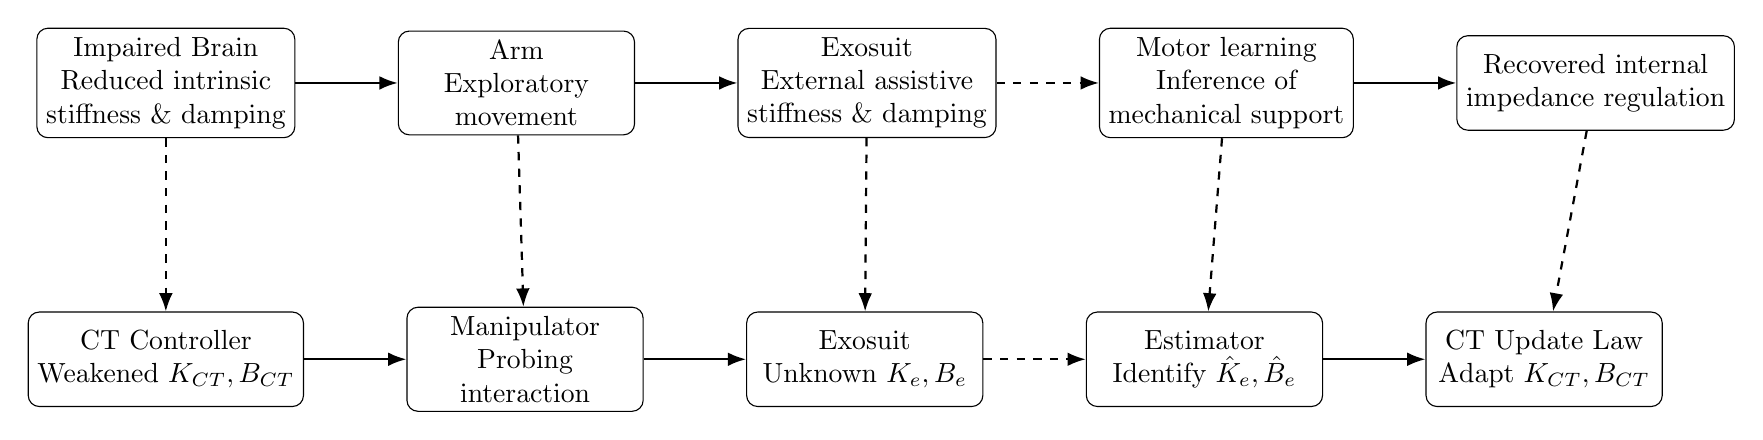
\begin{tikzpicture}[
    node distance=1.7cm and 1.3cm,
    block/.style={draw, rectangle, rounded corners, align=center, minimum width=3.0cm, minimum height=1.2cm},
    line/.style={-{Latex}, thick},
    dashedline/.style={-{Latex}, thick, dashed}
]

% Top row: biological analogy
\node[block] (brain) {Impaired Brain\\Reduced intrinsic\\stiffness \& damping};
\node[block, right=of brain] (arm) {Arm\\Exploratory\\movement};
\node[block, right=of arm] (bioexo) {Exosuit\\External assistive\\stiffness \& damping};
\node[block, right=of bioexo] (learn) {Motor learning\\Inference of\\mechanical support};
\node[block, right=of learn] (recover) {Recovered internal\\impedance regulation};

\draw[line] (brain) -- (arm);
\draw[line] (arm) -- (bioexo);
\draw[dashedline] (bioexo) -- (learn);
\draw[line] (learn) -- (recover);

% Bottom row: robotic analogy
\node[block, below=2.2cm of brain] (ct) {CT Controller\\Weakened \(K_{CT},B_{CT}\)};
\node[block, right=of ct] (manip) {Manipulator\\Probing\\interaction};
\node[block, right=of manip] (roboexo) {Exosuit\\Unknown \(K_e,B_e\)};
\node[block, right=of roboexo] (est) {Estimator\\Identify \(\hat{K}_e,\hat{B}_e\)};
\node[block, right=of est] (update) {CT Update Law\\Adapt \(K_{CT},B_{CT}\)};

\draw[line] (ct) -- (manip);
\draw[line] (manip) -- (roboexo);
\draw[dashedline] (roboexo) -- (est);
\draw[line] (est) -- (update);

% Vertical correspondence lines
\draw[dashedline] (brain) -- (ct);
\draw[dashedline] (arm) -- (manip);
\draw[dashedline] (bioexo) -- (roboexo);
\draw[dashedline] (learn) -- (est);
\draw[dashedline] (recover) -- (update);

\end{tikzpicture}
\caption{Analogy between biological post-stroke rehabilitation and the proposed robotic learning framework. The impaired brain corresponds to a CT controller with weakened impedance parameters. The exosuit acts both as assistance and as a teaching mechanism, whose estimated stiffness and damping are internalized into the controller.}
\label{fig:tikz_analogy}
\end{figure}

\begin{figure}[t]
\centering
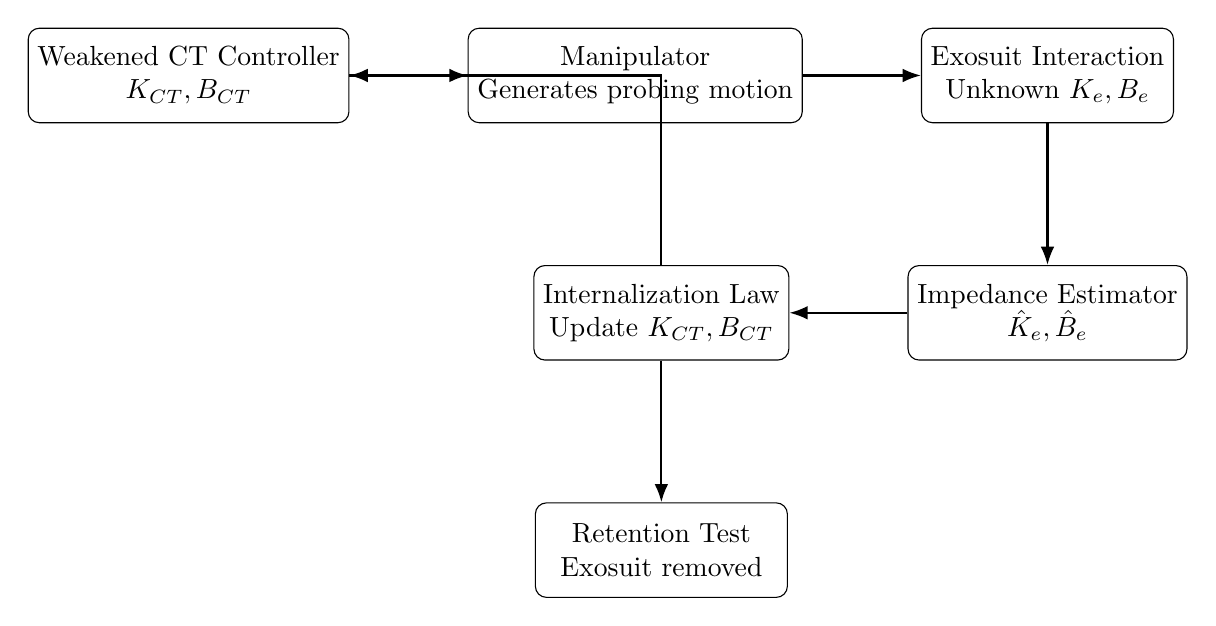
\begin{tikzpicture}[
    node distance=1.8cm and 1.5cm,
    block/.style={draw, rectangle, rounded corners, align=center, minimum width=3.2cm, minimum height=1.2cm},
    line/.style={-{Latex}, thick}
]

\node[block] (ct) {Weakened CT Controller\\\(K_{CT}, B_{CT}\)};
\node[block, right=of ct] (manip) {Manipulator\\Generates probing motion};
\node[block, right=of manip] (exo) {Exosuit Interaction\\Unknown \(K_e, B_e\)};
\node[block, below=of exo] (est) {Impedance Estimator\\\(\hat{K}_e, \hat{B}_e\)};
\node[block, left=of est] (upd) {Internalization Law\\Update \(K_{CT}, B_{CT}\)};
\node[block, below=of upd] (eval) {Retention Test\\Exosuit removed};

\draw[line] (ct) -- (manip);
\draw[line] (manip) -- (exo);
\draw[line] (exo) -- (est);
\draw[line] (est) -- (upd);
\draw[line] (upd) |- (ct);
\draw[line] (upd) -- (eval);

\end{tikzpicture}
\caption{Proposed rehabilitation-inspired robotic learning framework. A weakened CT controller drives the manipulator, which probes the exosuit. Estimated exosuit stiffness and damping are internalized into the CT controller, and retention is evaluated after exosuit removal.}
\label{fig:framework}
\end{figure}

\section{Reinforcement Learning for Probing Strategy}

\subsection{Motivation}

A key question in the proposed framework is how the manipulator should probe the exosuit in order to estimate its impedance efficiently, safely, and with minimal unnecessary effort. If the probing motion is too weak, the exosuit parameters may not be sufficiently excited for accurate estimation. If the probing motion is too aggressive, the interaction may become unsafe, energetically inefficient, or inconsistent with rehabilitation-inspired behavior.

We therefore formulate probing as a sequential decision-making problem and use reinforcement learning (RL) to learn an informative probing policy.

\subsection{Role of RL in the Framework}

In this framework, RL is not primarily used to replace the CT controller. Instead, RL determines the \emph{probing strategy}, that is, the exploratory motion or excitation pattern that the manipulator should generate in order to reveal the exosuit's effective stiffness and damping.

Thus:
\begin{itemize}
    \item the CT controller governs movement execution and impedance-based interaction,
    \item the estimator identifies exosuit parameters from measured data,
    \item the RL agent selects probing actions that improve parameter identifiability.
\end{itemize}

This interpretation is consistent with the rehabilitation analogy: the system learns \emph{how to explore assistance} in a way that reveals useful mechanical information.

\subsection{RL Formulation}

We model the probing problem as a Markov decision process (MDP) defined by states, actions, transition dynamics, and rewards.

\subsubsection{State Space}

The RL state should encode the current mechanical and estimation context. A suitable state vector is
\begin{equation}
s_t =
\begin{bmatrix}
q_t,\;
\dot{q}_t,\;
\hat{K}_e(t),\;
\hat{B}_e(t),\;
\mathrm{vec}(P_t),\;
e_t,\;
\tau_t
\end{bmatrix},
\label{eq:rl_state}
\end{equation}
where:
\begin{itemize}
    \item \(q_t\) is the joint angle,
    \item \(\dot{q}_t\) is the joint velocity,
    \item \(\hat{K}_e(t)\) and \(\hat{B}_e(t)\) are the current impedance estimates,
    \item \(P_t\) is the estimator covariance or uncertainty matrix,
    \item \(e_t\) is the task tracking error,
    \item \(\tau_t\) is the interaction torque.
\end{itemize}

If a lower-dimensional state is preferred, one may use
\begin{equation}
s_t = [q_t,\dot{q}_t,\hat{K}_e(t),\hat{B}_e(t),u_t],
\end{equation}
where \(u_t\) is a scalar uncertainty measure, such as \(u_t=\mathrm{tr}(P_t)\).

\subsubsection{Action Space}

The RL action determines the probing command. Several formulations are possible.

\paragraph{Amplitude-frequency probing.}
The agent selects the amplitude and frequency of a probing motion:
\begin{equation}
a_t = [A_t,\omega_t].
\end{equation}

A corresponding probing reference can be
\begin{equation}
q_{\mathrm{probe}}(t) = q_{\mathrm{ref}}(t) + A_t \sin(\omega_t t).
\label{eq:probe_signal}
\end{equation}

\paragraph{Torque-based probing.}
Alternatively, the agent directly selects an excitation torque:
\begin{equation}
a_t = \tau_{\mathrm{probe}}(t).
\end{equation}

\paragraph{Motion primitive selection.}
A more structured approach is to let the agent choose among predefined probing primitives, such as:
\begin{itemize}
    \item slow flexion-extension,
    \item sinusoidal oscillation,
    \item velocity pulse,
    \item small perturbation around equilibrium.
\end{itemize}

In that case, \(a_t\) indexes a discrete set of probing behaviors.

\subsubsection{Transition Dynamics}

The system evolves according to the manipulator dynamics, exosuit interaction, estimator updates, and CT controller response. RL does not require an explicit analytical transition model if a model-free method is used, but conceptually the dynamics are
\begin{equation}
s_{t+1} \sim p(s_{t+1}\mid s_t,a_t).
\end{equation}

The transition includes:
\begin{enumerate}
    \item application of probing action \(a_t\),
    \item physical interaction with the exosuit,
    \item collection of force-motion measurements,
    \item estimator update producing \(\hat{K}_e(t+1)\), \(\hat{B}_e(t+1)\), and \(P_{t+1}\).
\end{enumerate}

\subsection{Reward Design}

The probing policy should maximize information gain while minimizing unsafe or inefficient interaction. A suitable reward is
\begin{equation}
r_t =
\alpha\,\mathrm{InfoGain}_t
-\beta\,\|\tau_t\|^2
-\gamma\,\mathrm{SafetyCost}_t
-\delta\,\|e_t\|^2,
\label{eq:rl_reward_general}
\end{equation}
where:
\begin{itemize}
    \item \(\mathrm{InfoGain}_t\) rewards reduction in parameter uncertainty,
    \item \(\|\tau_t\|^2\) penalizes excessive probing effort,
    \item \(\mathrm{SafetyCost}_t\) penalizes unsafe motions or torque limits,
    \item \(\|e_t\|^2\) penalizes excessive deviation from the desired task.
\end{itemize}

A practical information-gain term is
\begin{equation}
\mathrm{InfoGain}_t = \mathrm{tr}(P_t)-\mathrm{tr}(P_{t+1}),
\label{eq:infogain_trace}
\end{equation}
so that reward is positive when estimator uncertainty decreases.

Thus, a more explicit reward becomes
\begin{equation}
r_t =
\alpha \bigl(\mathrm{tr}(P_t)-\mathrm{tr}(P_{t+1})\bigr)
-\beta \|\tau_t\|^2
-\gamma\,\mathrm{SafetyCost}_t
-\delta \|e_t\|^2.
\label{eq:rl_reward_trace}
\end{equation}

\subsection{Safety-Aware Reward Terms}

To ensure rehabilitation-consistent probing, safety penalties can be introduced when joint limits, velocity bounds, or torque bounds are violated. For example,
\begin{equation}
\mathrm{SafetyCost}_t =
c_q \,\mathbf{1}_{q_t \notin \mathcal{Q}}
+ c_{\dot{q}} \,\mathbf{1}_{\dot{q}_t \notin \mathcal{V}}
+ c_{\tau} \,\mathbf{1}_{\tau_t \notin \mathcal{T}},
\end{equation}
where:
\begin{itemize}
    \item \(\mathcal{Q}\) is the safe joint-angle range,
    \item \(\mathcal{V}\) is the safe velocity range,
    \item \(\mathcal{T}\) is the safe torque range.
\end{itemize}

A smooth alternative is to use quadratic barrier penalties:
\begin{equation}
\mathrm{SafetyCost}_t =
c_q \,\mathrm{dist}(q_t,\mathcal{Q})^2
+ c_{\dot{q}} \,\mathrm{dist}(\dot{q}_t,\mathcal{V})^2
+ c_{\tau} \,\mathrm{dist}(\tau_t,\mathcal{T})^2.
\end{equation}

\subsection{Objective of the RL Agent}

The RL agent learns a probing policy
\begin{equation}
\pi_\theta(a_t \mid s_t),
\end{equation}
parameterized by \(\theta\), that maximizes the expected discounted return
\begin{equation}
J(\theta)=\mathbb{E}_{\pi_\theta}\left[\sum_{t=0}^{T}\gamma_{\mathrm{RL}}^t r_t\right],
\end{equation}
where \(\gamma_{\mathrm{RL}}\in(0,1)\) is the RL discount factor.

The learned policy should therefore generate probing motions that:
\begin{itemize}
    \item excite the exosuit sufficiently to reveal \(K_e\) and \(B_e\),
    \item reduce estimator uncertainty quickly,
    \item avoid unsafe or overly large interactions,
    \item remain compatible with the CT-controlled movement objective.
\end{itemize}

\subsection{Connection to Parameter Estimation}

The RL policy improves the quality of collected data rather than directly estimating parameters itself. The parameter estimator still performs the identification step:
\begin{equation}
\hat{\theta}_{t+1} = \mathcal{E}(\hat{\theta}_t, y_t, \phi_t),
\end{equation}
where
\begin{equation}
\hat{\theta}_t =
\begin{bmatrix}
\hat{K}_e(t)\\
\hat{B}_e(t)
\end{bmatrix}.
\end{equation}

For instance, under recursive least squares,
\begin{equation}
\hat{\theta}_{t+1}
=
\hat{\theta}_t
+
L_t \bigl(y_t-\phi_t^\top \hat{\theta}_t\bigr),
\end{equation}
where \(L_t\) is the estimator gain.

Hence, RL and estimation play complementary roles:
\begin{itemize}
    \item RL chooses how to probe,
    \item the estimator computes what the exosuit parameters are from the resulting measurements.
\end{itemize}

\subsection{Recommended RL Algorithms}

Because the probing command is naturally continuous, suitable RL methods include:
\begin{itemize}
    \item Deep Deterministic Policy Gradient (DDPG),
    \item Twin Delayed DDPG (TD3),
    \item Soft Actor-Critic (SAC),
    \item Proximal Policy Optimization (PPO), if the probing command is parameterized suitably.
\end{itemize}

If the probing strategy is chosen from a finite set of motion primitives, discrete-action methods such as Deep Q-Networks (DQN) may also be used.

Among these, SAC is especially attractive because it balances reward maximization and exploration, which is valuable when informative probing requires persistent but safe exploration.

\subsection{Integration into the Full Framework}

The full loop with RL-based probing is:
\begin{enumerate}
    \item initialize weakened CT parameters \(K_{CT}, B_{CT}\),
    \item observe current state \(s_t\),
    \item RL policy selects probing action \(a_t\),
    \item manipulator executes the probing motion,
    \item exosuit interaction produces torque-motion data,
    \item estimator updates \(\hat{K}_e,\hat{B}_e\) and uncertainty \(P_t\),
    \item reward is computed from information gain, effort, safety, and task error,
    \item RL policy is updated,
    \item estimated exosuit parameters are used to update CT parameters.
\end{enumerate}

This closes the loop between exploration, identification, and internalization.

\subsection{Compact Summary Equation}

The overall probing-learning loop may be summarized as
\begin{equation}
a_t \sim \pi_\theta(\cdot \mid s_t),
\end{equation}
\begin{equation}
(q_t,\dot{q}_t,\tau_t) \longrightarrow (\hat{K}_e(t),\hat{B}_e(t),P_t),
\end{equation}
\begin{equation}
r_t =
\alpha \bigl(\mathrm{tr}(P_t)-\mathrm{tr}(P_{t+1})\bigr)
-\beta \|\tau_t\|^2
-\gamma\,\mathrm{SafetyCost}_t
-\delta \|e_t\|^2,
\end{equation}
\begin{equation}
K_{CT}(t+1)=K_{CT}(t)+\eta_K w_t \hat{K}_e(t),
\end{equation}
\begin{equation}
B_{CT}(t+1)=B_{CT}(t)+\eta_B w_t \hat{B}_e(t).
\end{equation}

This shows clearly that RL optimizes \emph{how to probe}, while the controller update determines \emph{how learned assistance is internalized}.

\subsection{Explanation of the Role of RL in the Probing Formulation}

In this framework, reinforcement learning (RL) is used to determine \emph{how the robot should probe the exosuit} so that the unknown impedance parameters can be identified efficiently and safely. The key idea is that probing is not treated as a fixed preprogrammed excitation, but as a sequential decision-making problem. At each time step, the agent observes the current mechanical state of the system, the present quality of the impedance estimates, and the interaction outcome, and then chooses the next probing action that is expected to be most informative.

Thus, the role of RL is not to replace the estimator or the CT controller. Instead, RL acts as a supervisory layer that selects informative probing actions. The estimator is still responsible for computing the parameter estimates \(\hat{K}_e(t)\), \(\hat{B}_e(t)\), and the uncertainty matrix \(P_t\), while the CT controller still governs the low-level tracking behavior. RL decides how to excite the system so that the estimator receives rich data without causing unsafe or unnecessarily aggressive interaction.

This is why the problem is modeled as a Markov decision process (MDP). The state \(s_t\) summarizes everything that is relevant for choosing the next probing action. It includes the current joint position \(q_t\) and velocity \(\dot q_t\), because the usefulness and safety of a probing action depend on the current motion condition. It also includes the current impedance estimates \(\hat K_e(t)\) and \(\hat B_e(t)\), because the probing strategy should depend on what the robot already believes about the exosuit. The covariance matrix \(P_t\), or a scalar uncertainty measure such as \(\mathrm{tr}(P_t)\), is especially important because it tells the agent how uncertain the current estimate is. If uncertainty is large, the agent should choose actions that generate more informative excitation. If uncertainty is already small, the agent may reduce probing intensity. The state also contains the tracking error \(e_t\) and interaction torque \(\tau_t\), which inform the agent whether the system is deviating too far from the desired task or producing excessive forces.

The action \(a_t\) represents the probing command selected by the RL agent. This action can be defined in different ways depending on the implementation. In the amplitude-frequency formulation, the agent chooses the probing amplitude \(A_t\) and frequency \(\omega_t\), which determine the excitation signal added to the nominal task trajectory:
\begin{equation}
q_{\mathrm{probe}}(t)=q_{\mathrm{ref}}(t)+A_t\sin(\omega_t t).
\end{equation}
In this case, RL learns whether the system should be excited gently or strongly, and whether slow or fast oscillations are more informative. In a torque-based formulation, the agent chooses a probing torque directly. In a discrete formulation, the agent selects one probing primitive from a library of safe behaviors, such as small oscillation, pulse excitation, or equilibrium perturbation. In all cases, the purpose of the action is the same: produce data that helps reveal the exosuit impedance.

The transition dynamics describe what happens after a probing action is applied. Once the agent chooses \(a_t\), the robot interacts physically with the exosuit, measurements are collected, and the estimator updates the learned parameters. Therefore, the next state \(s_{t+1}\) depends on the current state, the chosen probing action, the mechanical response of the system, and the estimation algorithm. Even if this mapping is not known analytically, RL can still learn from repeated interaction by observing which actions lead to better outcomes.

The reward function defines what constitutes a good probing decision. In this formulation, the reward encourages the agent to reduce estimation uncertainty while discouraging unsafe or wasteful probing. The term
\begin{equation}
\mathrm{InfoGain}_t=\mathrm{tr}(P_t)-\mathrm{tr}(P_{t+1})
\end{equation}
measures how much uncertainty has been reduced after taking action \(a_t\). If the covariance decreases significantly, the action has been informative, and the reward becomes larger. This is the central role of RL: to discover actions that maximize this uncertainty reduction. However, probing should not become arbitrarily large or aggressive. For this reason, the reward also penalizes the interaction torque \(\|\tau_t\|^2\), which discourages excessive excitation effort, and penalizes the tracking error \(\|e_t\|^2\), which ensures that probing remains compatible with the main movement task. The safety cost further penalizes actions that violate allowable position, velocity, or torque limits.

The safety terms are especially important in rehabilitation-inspired interaction, because the most informative probing action is not always the safest one. For example, a large high-frequency perturbation may reduce uncertainty quickly, but it may also generate uncomfortable torque peaks or drive the joint close to unsafe limits. RL therefore learns a compromise between informativeness and safety. This makes the probing policy adaptive: it seeks actions that are sufficiently exciting to identify the exosuit, but not so large that they interfere with rehabilitation objectives or patient comfort.

The objective function
\begin{equation}
J(\theta)=\mathbb{E}_{\pi_\theta}\left[\sum_{t=0}^{T}\gamma_{\mathrm{RL}}^t r_t\right]
\end{equation}
means that the agent does not optimize only the immediate reward at one time step, but the cumulative long-term benefit of its probing strategy. This is important because a probing action that is slightly costly now may be worthwhile if it greatly improves parameter estimates and leads to better future actions. The discount factor \(\gamma_{\mathrm{RL}}\) controls how strongly the agent values future rewards relative to immediate ones.

To illustrate the role of RL, consider the following example. Suppose the robot starts with a very uncertain estimate of exosuit stiffness and damping, so that \(P_t\) is large. In that case, the RL agent may choose a probing action with moderate amplitude and a frequency that excites the joint near the range where stiffness and damping effects are distinguishable. After the action is applied, the measured torque and motion data allow the estimator to reduce uncertainty, so that \(\mathrm{tr}(P_{t+1})<\mathrm{tr}(P_t)\). The reward is therefore positive. At a later stage, once the uncertainty becomes small and the tracking error begins to rise, the RL agent may reduce the probing amplitude or switch to a gentler probing primitive. In this way, the policy adapts over time: it probes aggressively when information is needed and cautiously when the estimate is already reliable.

In summary, the role of RL in this formulation is to learn an adaptive probing policy that balances four competing goals:
\begin{enumerate}
    \item excite the exosuit enough to reveal its stiffness and damping,
    \item reduce estimator uncertainty as quickly as possible,
    \item avoid unsafe joint motion and excessive interaction torque,
    \item preserve compatibility with the CT-controlled rehabilitation task.
\end{enumerate}
Therefore, RL serves as the intelligent exploration mechanism of the framework. It decides how to generate informative excitation, while the estimator converts the resulting data into impedance estimates and the controller uses those estimates for internalization.




\pagebreak 
\section{Probable Approaches Given the Current Implementation}
The system is already far enough along in the repository that the next step does not need to be ``build the model from scratch.''  A more useful framing is to choose which scientific claim to pursue first.  The existing implementation supports several plausible paths.

\subsection{Approach 1: Direct Impedance-Shaping Evidence}
This is the most immediate path.  Use the implemented PyDrake exosuit model in the main tendon-with-exo PyDrake script
\begin{center}
\small\texttt{script\_cup\_manipulator\_pendulam\_tendon\_with\_exo\_pydrake.py}
\end{center}
and the existing VS Code tasks for exo ON/OFF, disturbance-synchronized, and reactive activation.

The core experiment is:
\begin{align}
    \tau_{\mathrm{exo}} &\approx -K_{\mathrm{exo,eff}}(q_2-q_{2,a}) - D_{\mathrm{exo,eff}}\dot{q}_2, \\
    K_{\mathrm{exo,eff}} &= 2k_{\mathrm{exo}}r_{\mathrm{exo}}^2, \qquad
    D_{\mathrm{exo,eff}} = 2b_{\mathrm{exo}}r_{\mathrm{exo}}^2 .
\end{align}
Compare tracking and disturbance rejection under identical axes for:
\begin{itemize}[leftmargin=1.5em]
    \item exo off / transparent baseline,
    \item exo on during the disturbance window,
    \item reactive exo activation triggered by tracking error,
    \item multiple trajectories: circle, rectangle, figure-eight, and line.
\end{itemize}

The likely first claim is modest but defensible: the exosuit behaves like a programmable impedance layer that improves disturbance rejection and produces a clearer state-force relationship.  This path is best for a first result because it is already implemented, easy to visualize, and does not require proving a global learning theorem.

\subsection{Approach 2: Parameter-Identification View of Learning}
The second path treats the exosuit as something the controller/human can probe.  From logged trajectories, estimate effective stiffness and damping by fitting
\begin{equation}
    \tau_{\mathrm{int}}(t) \approx -\hat{K}\,(q_2(t)-q_{2,a}) - \hat{D}\,\dot{q}_2(t).
\end{equation}
Then use the estimates to update a weak controller:
\begin{align}
    K_{P,t+1} &= K_{P,t} + \eta_K(\hat{K}-K_{P,t}), \\
    K_{D,t+1} &= K_{D,t} + \eta_D(\hat{D}-K_{D,t}).
\end{align}

This is not meant to claim that the brain literally estimates numerical gains.  Rather, it provides an engineering analogue for the rehabilitation idea: repeated interaction with a structured impedance can create a more learnable feedback signal.  This approach is especially useful if the paper is framed around motor learning or rehabilitation rather than pure controller synthesis.

\subsection{Approach 3: Local Contraction / CCM Certification}
The contraction-theory implementation already includes MATLAB scripts for comparing no-exo and with-exo cases:
\begin{itemize}[leftmargin=1.5em]
    \item \texttt{script\_14e\_cupex\_CCM\_block\_LMI\_no\_exo.m},
    \item \texttt{script\_14f\_cupex\_CCM\_block\_LMI\_with\_exo.m},
    \item \texttt{script\_14g\_cupex\_CCM\_original.m}.
\end{itemize}
This path asks whether the passive exosuit terms make the linearized or sampled nonlinear dynamics easier to certify as contracting.  Conceptually, the exo adds negative stiffness/damping-like terms to the elbow dynamics, so the certified contraction rate may improve:
\begin{equation}
    \lambda_{\max}^{\mathrm{exo}} > \lambda_{\max}^{\mathrm{no\;exo}}.
\end{equation}

This is the cleanest theory-facing approach.  The limitation is that the result is local or sampled over a chosen region, not a universal statement about all human-exosuit behavior.  That limitation is acceptable if stated clearly: the exosuit increases the size or strength of a certifiable stable region around the task dynamics.

\subsection{Approach 4: C3M Residual Controller on Top of Computed Torque}
The C3M path is already represented by the PyTorch systems and MATLAB deployment scripts:
\begin{itemize}[leftmargin=1.5em]
    \item \texttt{C3M/systems/system\_CUPMANIP\_SEA\_EXO\_TRACK.py},
    \item \texttt{C3M/systems/system\_CUPMANIP\_SEA\_EXO\_LINEXO.py},
    \item \texttt{script\_14h\_cupex\_C3M\_SEA\_exo.m},
    \item \texttt{script\_14i\_cupex\_C3M\_exo\_embedded.m}.
\end{itemize}
The practical insight from today is that the raw input matrix can be state-dependent through the manipulator inertia.  The constant-\(B\) C3M variants freeze \(B\) at the operating point so that the difficult C2 compatibility term is removed from the training burden:
\begin{equation}
    B(x) \rightarrow B(x_\ast), \qquad \frac{\partial B}{\partial x}=0.
\end{equation}

The likely role of C3M in the near term is not to replace computed torque completely.  A safer use is as a residual stabilizing policy around a known baseline:
\begin{equation}
    u(t) = u_{\mathrm{CT}}(t) + u_{\mathrm{C3M}}(x(t),x_\ast(t)).
\end{equation}
This approach can answer whether learned contraction-style feedback improves robustness beyond CT alone.  It is higher risk than Approach 1 or 3 because training/deployment mismatch, motor-state chatter, and residual scaling can dominate the result.

\subsection{Approach 4b: AI / RL / Learning-Based Implementation Options}
AI and learning methods should be used as structured add-ons to the model-based controller, not as an immediate replacement for the physics.  The repository already contains the right starting points: the Isaac Sim PPO residual environment in \texttt{rl/envs/manipulator\_residual\_env.py}, the training script \texttt{rl/train\_ppo\_residual.py}, the evaluator \texttt{rl/eval\_ppo\_residual.py}, and the MATLAB scaffold \texttt{script\_14d\_cupex\_RL\_residual.m}.

The safest learning architecture is residual learning:
\begin{equation}
    \tau_{\mathrm{cmd}}(t)
    = \tau_{\mathrm{CT}}(t) + \Delta\tau_\theta(o_t),
    \qquad
    \|\Delta\tau_\theta\|_\infty \leq \tau_{\mathrm{res,max}} .
\end{equation}
Here CT remains the stabilizing backbone, while the learned policy handles effects that are hard to model exactly: SEA phase lag, cable slack/compliance, friction, unmodelled exo coupling, and trajectory-dependent tracking error.

The implemented RL observation already has a useful structure:
\begin{equation}
    o_t = [q_1,q_2,\dot{q}_1,\dot{q}_2,e_x,e_y,\delta,\dot{\delta},F_c,
           \tau_{2,\mathrm{CT}},\tau_{2,\mathrm{SEA}},\tau_m,
           e_{\tau_1},e_{\tau_2}]^\top .
\end{equation}
This observation is appropriate because it includes not only kinematic tracking error, but also the actuator-side quantities that reveal why CT may fail: spring extension, cable force, applied torque, motor torque, and torque-tracking error.

Several learning routes are plausible:
\begin{enumerate}[leftmargin=1.5em]
    \item \textbf{Residual PPO policy.}  Train \(\Delta\tau_\theta\) with PPO in Isaac Sim.  Reward should penalize EE error, residual effort, acceleration/smoothness, and torque-tracking mismatch:
    \begin{equation}
        r_t = -w_e\|e_{\mathrm{EE}}\|^2
              -w_u\|\Delta\tau_\theta\|^2
              -w_a\|\ddot{q}\|^2
              -w_\tau\|\tau_{\mathrm{des}}-\tau_{\mathrm{applied}}\|^2 .
    \end{equation}
    This is the most direct use of the existing \texttt{rl/} code.

    \item \textbf{Gain adaptation policy.}  Instead of outputting torque directly, learn a slower policy that adjusts impedance or controller gains:
    \begin{equation}
        [K_P,K_D,K_{\mathrm{exo}},D_{\mathrm{exo}}]_{t+1}
        = [K_P,K_D,K_{\mathrm{exo}},D_{\mathrm{exo}}]_t
          + \Delta_\theta(o_t).
    \end{equation}
    This is more interpretable for the rehabilitation story because the learned action changes ``how stiff'' and ``how damped'' the interaction feels rather than injecting arbitrary torque.

    \item \textbf{Learned exo activation policy.}  Replace hand-coded timed/reactive activation with a classifier or policy:
    \begin{equation}
        a_{\mathrm{exo}}(t) \in \{0,1\}, \qquad
        \Delta\theta_{\mathrm{exo}}(t) = \pi_\theta(o_t).
    \end{equation}
    This would learn when assistance should turn on, how much co-contraction offset to apply, and when to return to transparent mode.

    \item \textbf{Supervised imitation from an oracle.}  Generate data from CT, CCM, or hand-tuned exo-on/off experiments and train a smaller policy to imitate the best action.  This can be lower variance than RL and gives a clear baseline before PPO.

    \item \textbf{System-identification network.}  Learn \(\hat{K},\hat{D}\), friction, or SEA lag parameters from trajectory windows, then feed those estimates into a model-based controller.  This keeps the learned model interpretable and directly tied to the meeting hypothesis.

    \item \textbf{Offline model-based learning.}  Use simulation logs to fit a disturbance or residual dynamics model
    \begin{equation}
        x_{t+1} \approx f_{\mathrm{model}}(x_t,u_t) + d_\theta(x_t,u_t),
    \end{equation}
    then use the learned residual model for MPC, gain scheduling, or safer policy search.
\end{enumerate}

The recommended implementation order is conservative:
\begin{enumerate}[leftmargin=1.5em]
    \item run CT-only and CT+exo baselines first,
    \item train residual PPO with small torque bounds and compare against CT-only,
    \item add exo-aware observations and reward terms if the policy ignores cable/exo lag,
    \item move from torque residuals to gain/impedance adaptation for interpretability,
    \item finally test learned exo activation and catch-trial after-effects.
\end{enumerate}
The paper framing should emphasize that AI is a tool for discovering or tuning the feedback-shaping rule.  The scientific claim remains physical: the exosuit creates a structured impedance channel; learning methods determine how to use that channel effectively.

\subsection{Approach 5: Full Coupled Exosuit-State Certification}
The most physically faithful C3M path is the full augmented-state model, represented by
\begin{center}
\small\texttt{C3M/systems/system\_CUPMANIP\_SEA\_EXO\_FULL.py}\quad and\quad
\small\texttt{script\_14j\_cupex\_C3M\_exo\_full.m}.
\end{center}
Here the exo motor states are included in the learning/certification state, e.g.
\begin{equation}
    x_{10} = [q_1,q_2,\dot{q}_1,\dot{q}_2,\theta_m,\dot{\theta}_m,
              \theta_{mR},\dot{\theta}_{mR},\theta_{mL},\dot{\theta}_{mL}]^\top .
\end{equation}
This avoids pretending that the exosuit is only an algebraic spring-damper torque.  The tradeoff is complexity: the network is larger, the training problem is harder, and the explanation is less transparent.  This should probably be treated as a later robustness check, not the first paper's main result.

\subsection{Approach 6: Human / Rehabilitation Translation}
Once the simulation story is stable, the human-facing interpretation can be tested with catch-trial logic.  The simulation analogue is:
\begin{enumerate}[leftmargin=1.5em]
    \item Train or adapt the weak controller with exo impedance active.
    \item Remove or reduce the exo impedance suddenly.
    \item Check whether the controller shows an after-effect or retained compensation.
\end{enumerate}
In a human study, the same logic would ask whether participants adapt their motion after repeated exposure to a structured exosuit impedance.  This is the strongest rehabilitation framing, but it should come after the simulation has a clean effect size and a clear mechanistic story.

\subsection{Recommended Order}
The lowest-risk path is:
\begin{enumerate}[leftmargin=1.5em]
    \item establish exo ON/OFF disturbance-rejection plots with identical axes,
    \item quantify RMS error, peak error, settling time, and effective damping,
    \item run the CCM no-exo vs with-exo comparison to support the stability interpretation,
    \item add the parameter-identification story as the bridge to learning,
    \item use C3M residual control only after the baseline and CCM results are clean,
    \item reserve full 10D exo-state C3M and human catch trials as later-stage validation.
\end{enumerate}

Therefore, the probable first paper should not overclaim that the exosuit directly teaches the brain an exact \(K_P,K_D\) controller.  A stronger and more defensible claim is: a programmable exosuit can shape interaction impedance, improve local stability/disturbance rejection, and provide an interpretable physical channel that can be used for controller adaptation or rehabilitation-oriented learning.

\section{Open Conceptual Challenge}
One of the biggest unresolved questions was:

\begin{quote}
How exactly do we map the exosuit-provided physical feedback into a useful internal adaptation of the controller/brain?
\end{quote}

Several versions of the challenge were discussed:
\begin{itemize}[leftmargin=1.5em]
    \item exosuit impedance is not the same thing as neural control gains,
    \item parameter estimates do not directly explain perception,
    \item a strong engineering mapping may not align with human interpretation,
    \item and there may need to be an intermediate representation or ``language'' between the two domains.
\end{itemize}

This was variously described as:
\begin{itemize}[leftmargin=1.5em]
    \item a mapping problem,
    \item an interface problem,
    \item a representation problem,
    \item or even a ``language'' problem.
\end{itemize}

One tentative practical compromise discussed was:
\begin{itemize}[leftmargin=1.5em]
    \item initially assume a simple direct mapping from learned exosuit parameters to controller parameter changes,
    \item use that for simulation,
    \item and improve the interpretation layer later.
\end{itemize}

\section{Potential Role of AI / Learning Methods}
There was brief discussion of whether modern AI or learning-based methods might help.

Possible directions mentioned included:
\begin{itemize}[leftmargin=1.5em]
    \item reinforcement learning,
    \item data-driven adaptation,
    \item human-in-the-loop learning,
    \item and behavioral modeling.
\end{itemize}

However, this appeared exploratory rather than a final decision. There was also caution about:
\begin{itemize}[leftmargin=1.5em]
    \item complexity,
    \item interpretability,
    \item and whether a simpler model-based route should be tried first.
\end{itemize}

\section{Short-Term Technical Action Items}
The following near-term tasks were either explicitly stated or strongly implied:

\begin{enumerate}[leftmargin=1.5em]
    \item \textbf{Simplify the disturbance input:} replace sinusoidal disturbance with a step or pulse for clearer interpretation.
    \item \textbf{Overlay plots:} compare exosuit on/off responses on the same axes.
    \item \textbf{Check scaling:} ensure differences are not due to inconsistent plot scales.
    \item \textbf{Add omitted model components:} include any missing passive/mechanical terms if needed.
    \item \textbf{Build a toy coupled-system model:} represent the arm/controller and exosuit as interacting second-order systems.
    \item \textbf{Probe parameter regression:} test whether exosuit stiffness/damping can be estimated from interaction data.
    \item \textbf{Map identified parameters to weak controller gains:} try a simple heuristic update rule first.
    \item \textbf{Test critical-damping target behavior:} see whether the system can learn or be driven toward critically damped response.
    \item \textbf{Clarify contraction-control role:} decide whether contraction is central theory, supporting intuition, or only a local design tool.
\end{enumerate}

\section{Possible Paper Directions}
There was some discussion about publication strategy and what the first paper should actually claim.

Possible paper angles include:

\subsection{Paper Angle A: Formulation / Theory}
Focus on:
\begin{itemize}[leftmargin=1.5em]
    \item the hypothesis that exosuit-shaped impedance provides a learning-friendly feedback channel,
    \item mathematical formulation,
    \item simplified analysis,
    \item and simulation evidence.
\end{itemize}

\subsection{Paper Angle B: Design / Platform}
Focus on:
\begin{itemize}[leftmargin=1.5em]
    \item exosuit mechanism,
    \item cable-based stiffness modulation,
    \item and use as a programmable rehabilitation interface.
\end{itemize}

\subsection{Paper Angle C: Simulation + Human Pilot}
Focus on:
\begin{itemize}[leftmargin=1.5em]
    \item simulation formulation,
    \item parameter learning idea,
    \item and preliminary human testing or catch trials.
\end{itemize}

There was also discussion of aiming for a submission before the end of the year / before Christmas, with some uncertainty about venue and risk.

\section{Notes on Unclear Terms from the Transcript}
A few transcript fragments were likely corrupted or ambiguous. The following are \textbf{best-effort interpretations}:

\begin{itemize}[leftmargin=1.5em]
    \item ``KPKD'' was interpreted as proportional/derivative gain discussion.
    \item ``CCM'' was interpreted as control contraction metrics.
    \item ``residual controller'' appears to refer to an additional controller layered over an existing baseline controller.
    \item ``computer talk'' likely meant \emph{computed torque}.
    \item ``contraction region'' likely referred to learning or operating in a stable/convergent regime.
    \item ``back drivable mode'' appears to refer to exosuit transparency or low-impedance interaction mode.
\end{itemize}

\section{Non-Technical / Lab Logistics}
The meeting also included unrelated but important practical discussion:

\subsection{Workspace and Lab Setup}
\begin{itemize}[leftmargin=1.5em]
    \item There was interest in making the space feel like a proper lab.
    \item Whiteboards were suggested as useful additions.
    \item A possible count/arrangement of desks and available space was discussed.
    \item It was noted that more visible whiteboard space might help technical discussion and engagement.
\end{itemize}

\subsection{Meeting Room}
\begin{itemize}[leftmargin=1.5em]
    \item A nearby meeting room was mentioned.
    \item It appears to be bookable.
    \item Its location was described relative to the office entrance.
\end{itemize}

\subsection{Miscellaneous Side Conversation}
There were also short unrelated fragments about:
\begin{itemize}[leftmargin=1.5em]
    \item printing/layout issues,
    \item fish/shrimp setup,
    \item kitchen/lab usage,
    \item and general office organization.
\end{itemize}

These do not appear central to the technical project.

\section{Concise Summary}
In compact form, the meeting's technical direction can be summarized as follows:

\begin{enumerate}[leftmargin=1.5em]
    \item Model the human/controller as a weak dynamical system.
    \item Model the exosuit as providing programmable impedance (stiffness/damping).
    \item Let the controller interact with the exosuit and observe force/state relationships.
    \item Estimate or infer the exosuit dynamics from this interaction.
    \item Use that interaction as a structured feedback signal to guide controller adaptation.
    \item Test whether this creates faster or more stable learning than unaided interaction.
    \item Connect the result to rehabilitation: the exosuit may both assist movement and improve re-learning.
\end{enumerate}

\section{Immediate Next-Step Version}
A minimal actionable version of the plan is:

\begin{enumerate}[leftmargin=1.5em]
    \item Use a simple second-order toy model.
    \item Add exosuit stiffness and damping.
    \item Apply a step disturbance.
    \item Compare responses with exosuit on/off.
    \item Attempt parameter identification from interaction data.
    \item Use identified values to heuristically update weak controller gains.
    \item Check whether the result moves the system toward a more critically damped response.
\end{enumerate}

\section*{End Note}
These notes reflect a cleaned, structured reconstruction of a noisy conversation. They are suitable as a working record, but any equations, terminology, and paper claims should be refined against the actual model and code implementation.


\end{document}